\section{Auswertung}
\label{sec:Auswertung}
\subsection{Stabilitätsbedingung und das Frequenzspektrum}
Für diesen Versuch 
\begin{table}[h]
    \centering
    \caption{Graphisch ermittelte Länge der Gittervektoren des ersten Graphitscans.}
    \label{tab:Graphit_Bild_1}
    \begin{tblr}{colspec= c c c c}
        \toprule
        $\left|\vec{g}_{\text{1,vor}} \right| / \unit{\pico\meter}$ & $\left|\vec{g}_{\text{2,vor}} \right| / \unit{\pico\meter}$ & $\left|\vec{g}_{\text{1,rück}} \right| / \unit{\pico\meter}$ & $\left|\vec{g}_{\text{2,rück}}\right| / \unit{\pico\meter}$ \\
        \midrule
        $276,1  \pm 12,8$   & $175,1  \pm  5,1$    &  $277,6   \pm  5,1$   & $173,2    \pm 5,1$ \\
        $278,0  \pm 4,3 $   & $169,6  \pm  2,8$    &  $272,4   \pm  8,5$   & $171,5    \pm 6,4$ \\
        $274,1  \pm 6,4 $   & $169,3  \pm  3,2$    &  $273,3   \pm  4,3$   & $170,8    \pm 2,8$ \\
        $274,0  \pm 5,1 $   & $173,3  \pm  6,4$    &  $278,0   \pm  4,3$   & $171,5    \pm 2,8$ \\
        \bottomrule
    \end{tblr}
\end{table}

\begin{figure}[h]
    \centering
    \begin{subfigure}{.475\linewidth}
      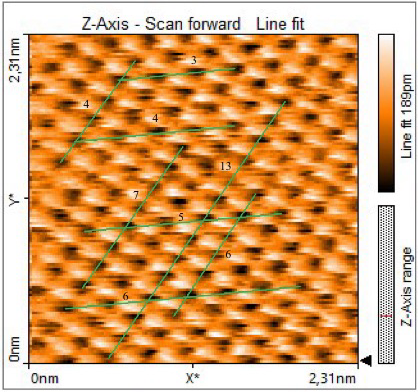
\includegraphics[width=\linewidth]{Messdaten/Gitter_Graphit/2_Bild_forwards.png}
    \end{subfigure}\hfill 
    \begin{subfigure}{.475\linewidth}
      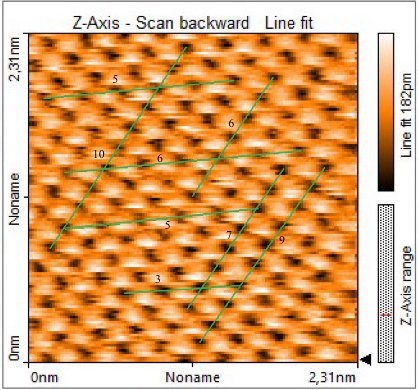
\includegraphics[width=\linewidth]{Messdaten/Gitter_Graphit/2_Bild_backwards.png}
    \end{subfigure}
    \caption{Zweiter Scan der Gitterstruktur von HOPG mit graphischer Auswertung.}
    \label{fig:Gitter_Graphit_2}
\end{figure}

% \begin{figure}
%   \centering
%   \includegraphics{plot.pdf}
%   \caption{Plot.}
%   \label{fig:plot}
% \end{figure}

%Siehe \autoref{fig:plot}!